\section{Visualisations - Champ électromagnétique}

Les figures ci-dessous montrent les parties réelle
et imaginaire du champ électromagnétique dans l'enceinte du four vide,
et dans l'enceinte du four avec l'aliment dedans.

La source du champ magnétique se trouve à gauche dans toutes les
figures, et on impose ici $g = 0$ sur toutes les autres parois
du four.

Voir les sections~\ref{experiences_numeriques:constantes}
et~\ref{experiences_numeriques:dimensions_four} pour consulter
les valeurs des paramètres physiques et les dimensions du four.

\subsection{Four vide}

\begin{figure}[H]
    \centering
    \begin{subfigure}{.5\textwidth}
        \centering
        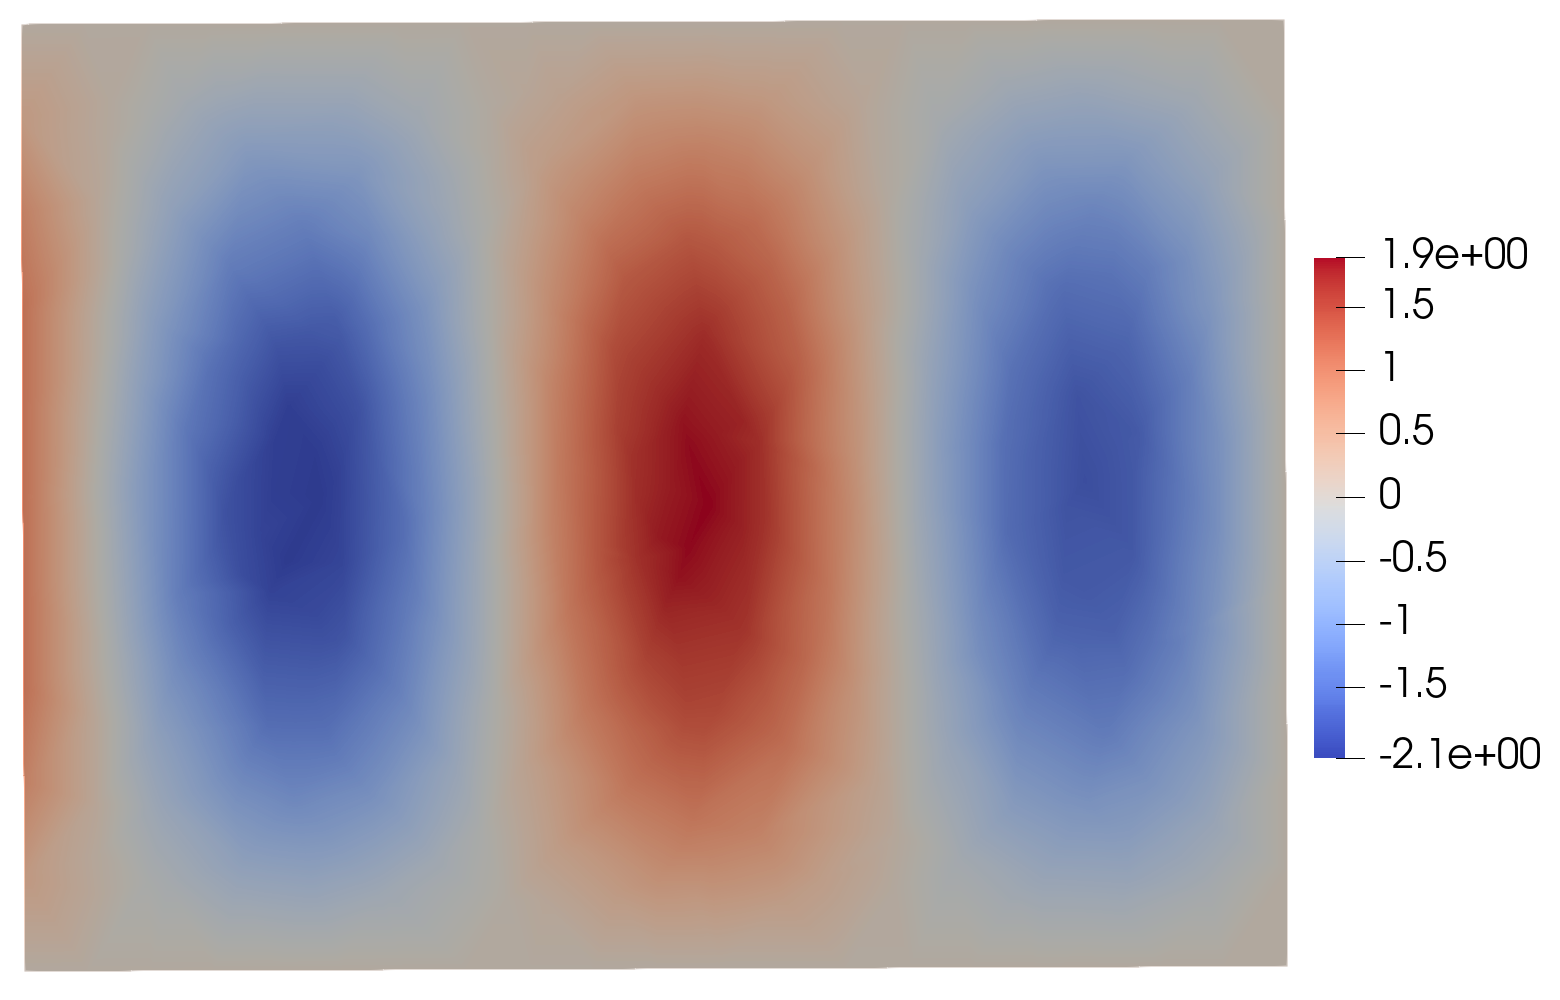
\includegraphics[scale=0.15]{figures/helmholtz/helmholtz_reel_vide1.png}
        \caption{Partie réelle}
    \end{subfigure}%
    \begin{subfigure}{.5\textwidth}
        \centering
        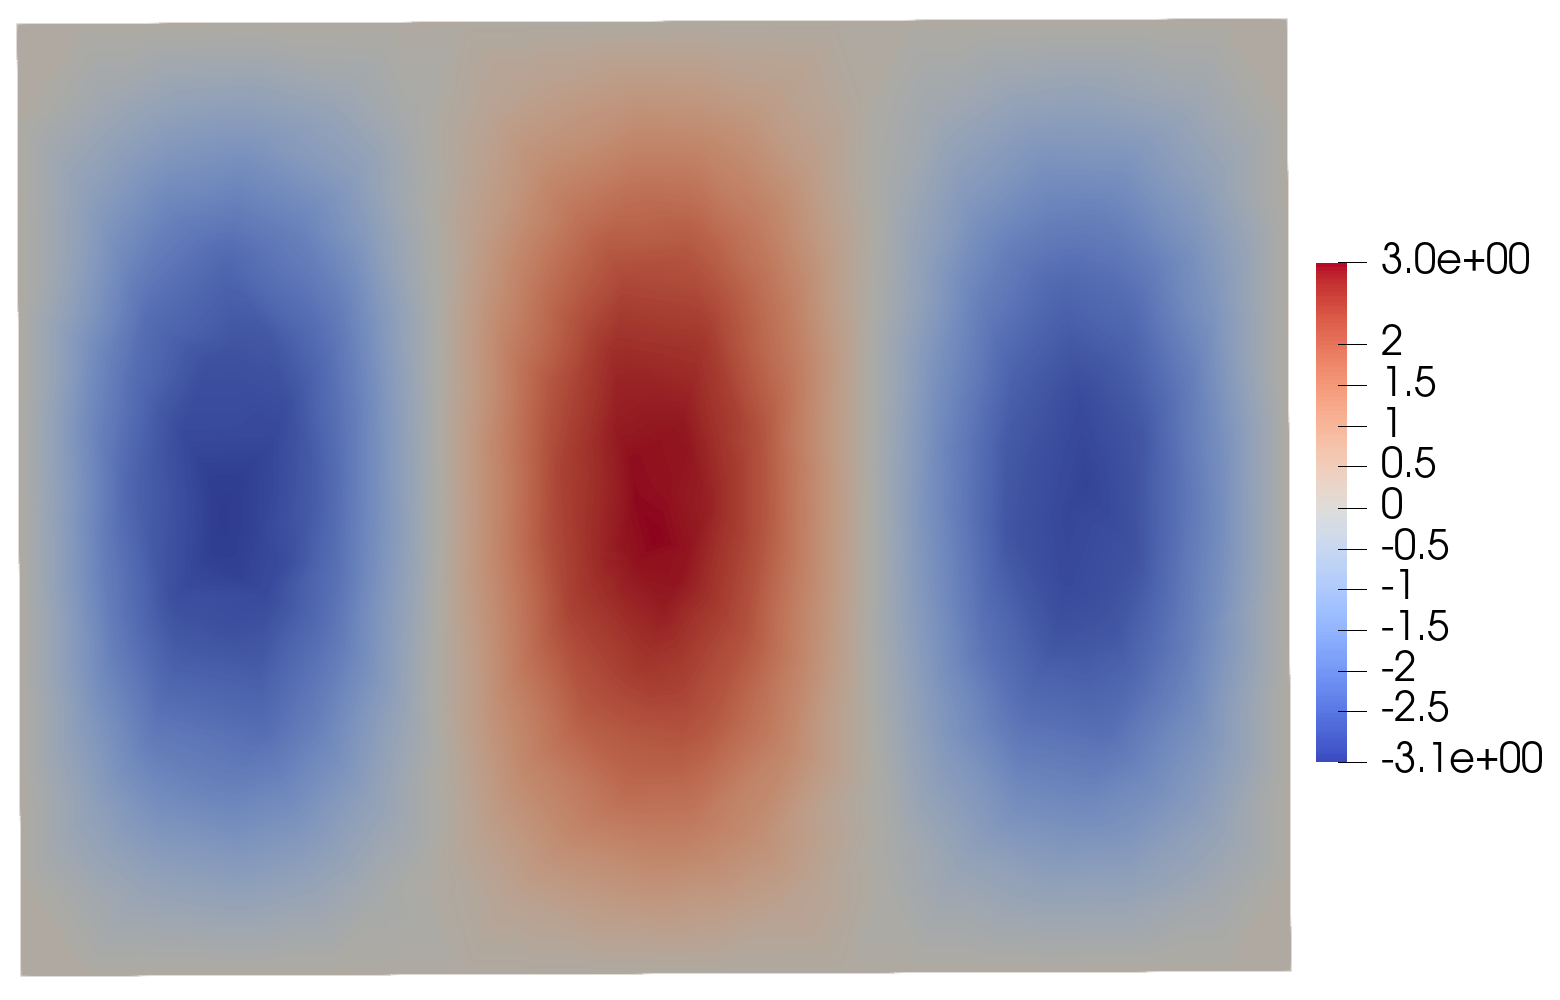
\includegraphics[scale=0.15]{figures/helmholtz/helmholtz_imag_vide1.png}
        \caption{Partie imaginaire}
    \end{subfigure}
    \caption{Une tranche de la magnitude du champ électromagnétique dans l'enceinte
    du four vide. La tranche est orientée selon l'axe $x$.}
\end{figure}

\begin{figure}[H]
    \centering
    \begin{subfigure}{.5\textwidth}
        \centering
        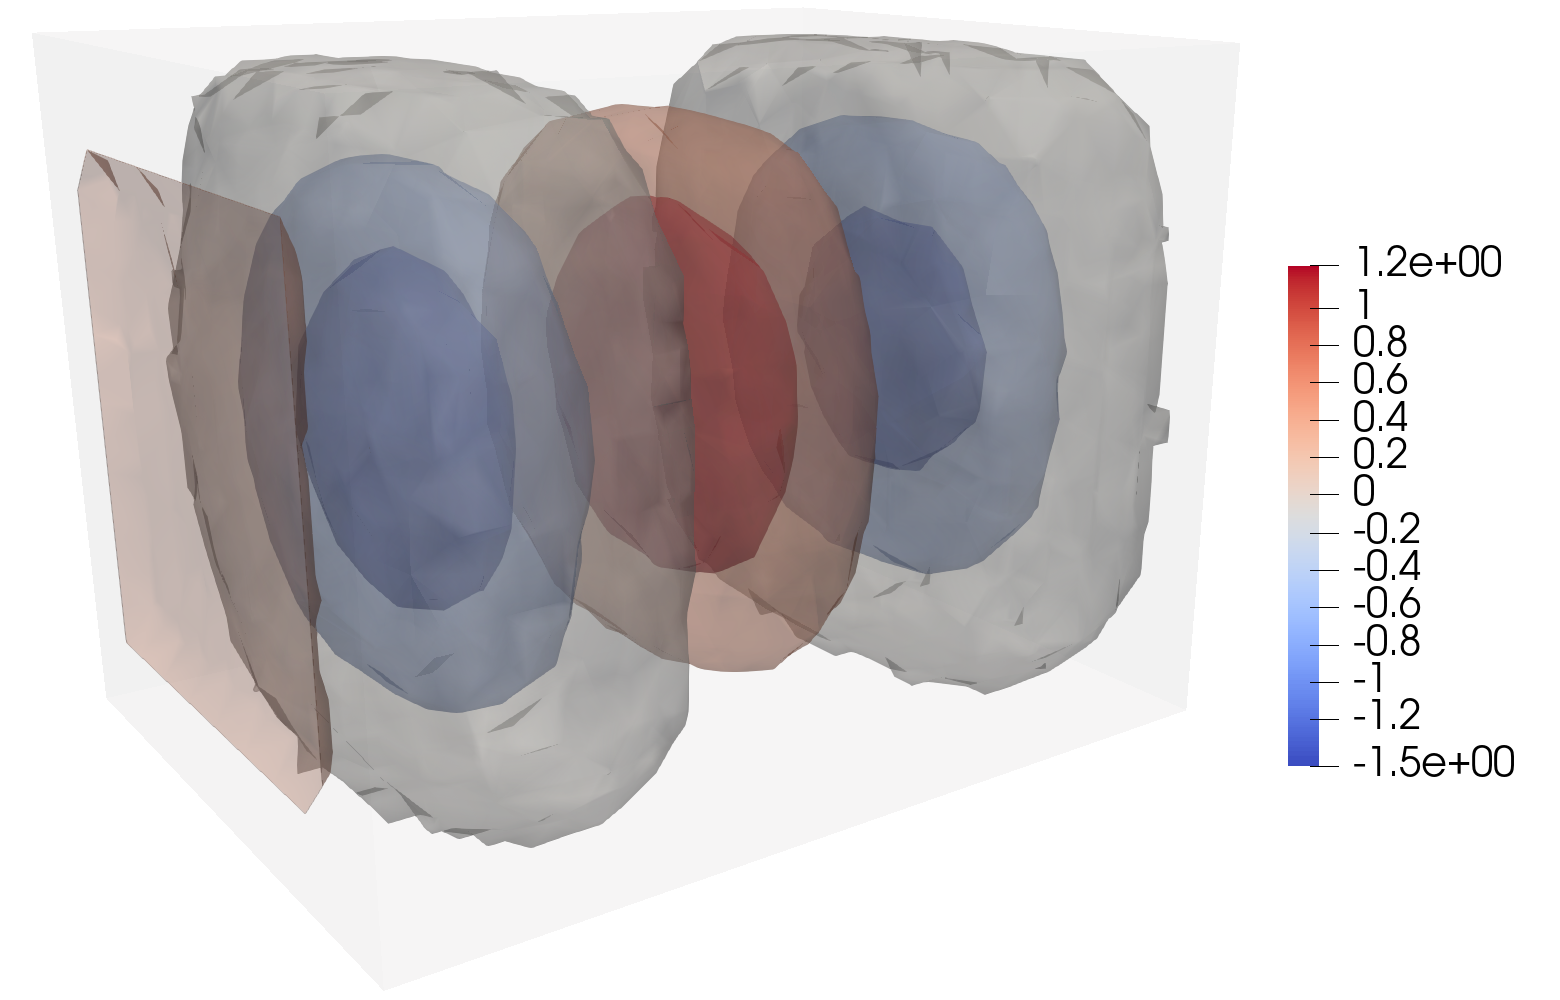
\includegraphics[scale=0.15]{figures/helmholtz/helmholtz_reel_vide2.png}
        \caption{Partie réelle}
    \end{subfigure}%
    \begin{subfigure}{.5\textwidth}
        \centering
        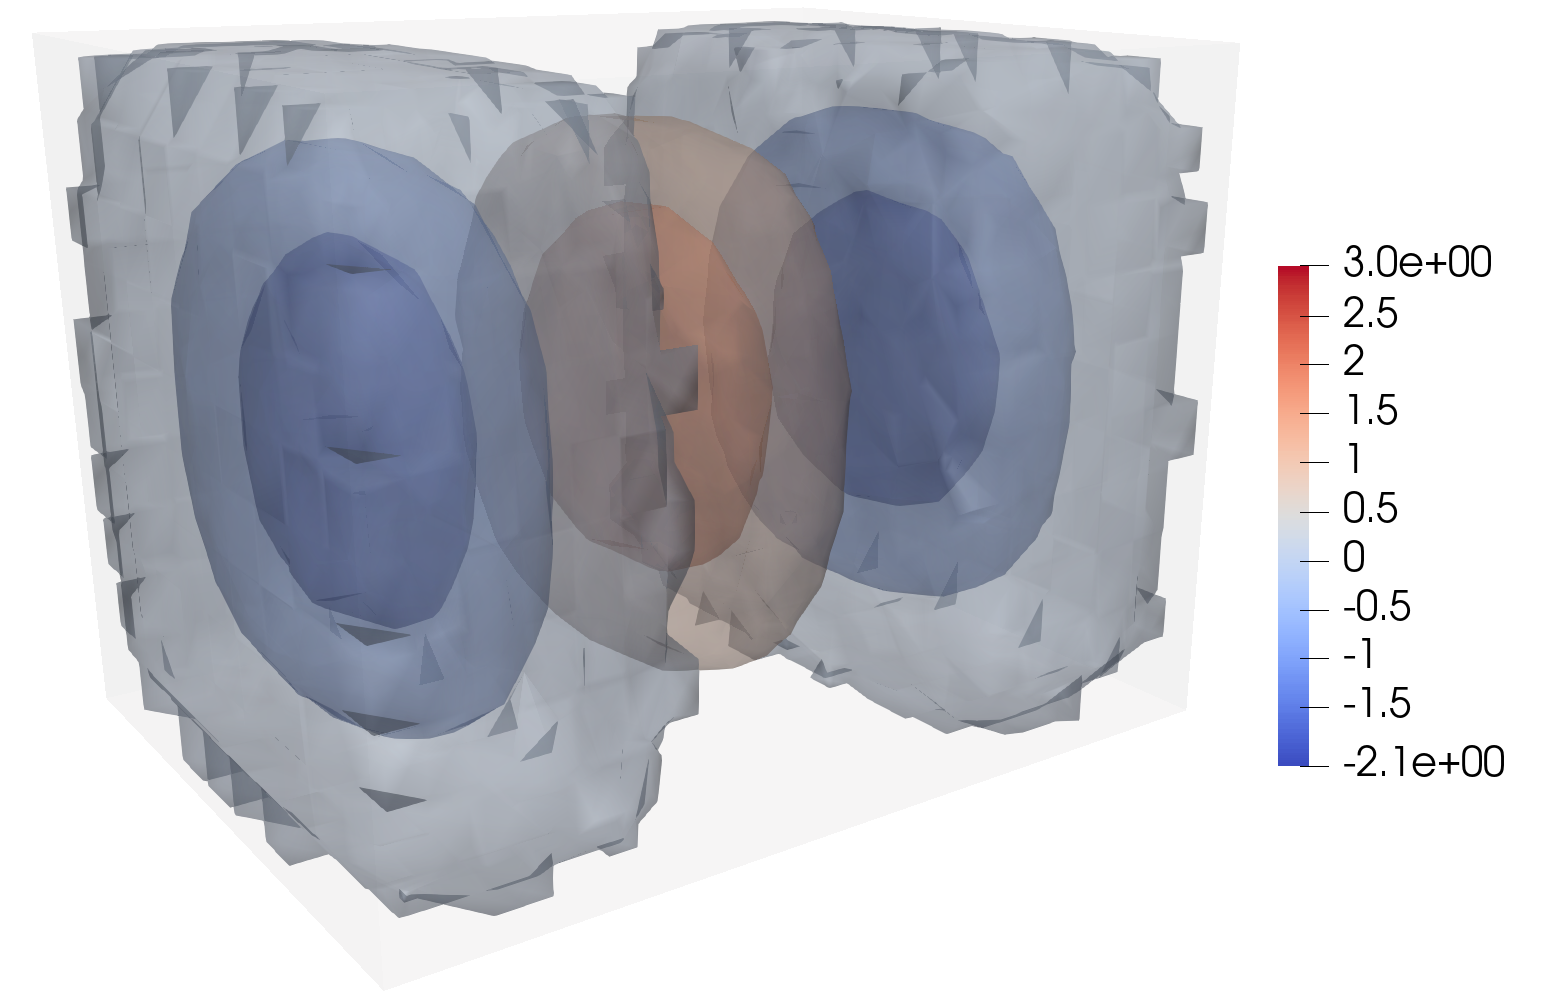
\includegraphics[scale=0.15]{figures/helmholtz/helmholtz_imag_vide2.png}
        \caption{Partie imaginaire}
    \end{subfigure}
    \caption{Des tracés de contours de la magnitude du champ électromagnétique
    dans l'enceinte du four vide.}
\end{figure}

\begin{figure}[H]
    \centering
    \begin{subfigure}{.5\textwidth}
        \centering
        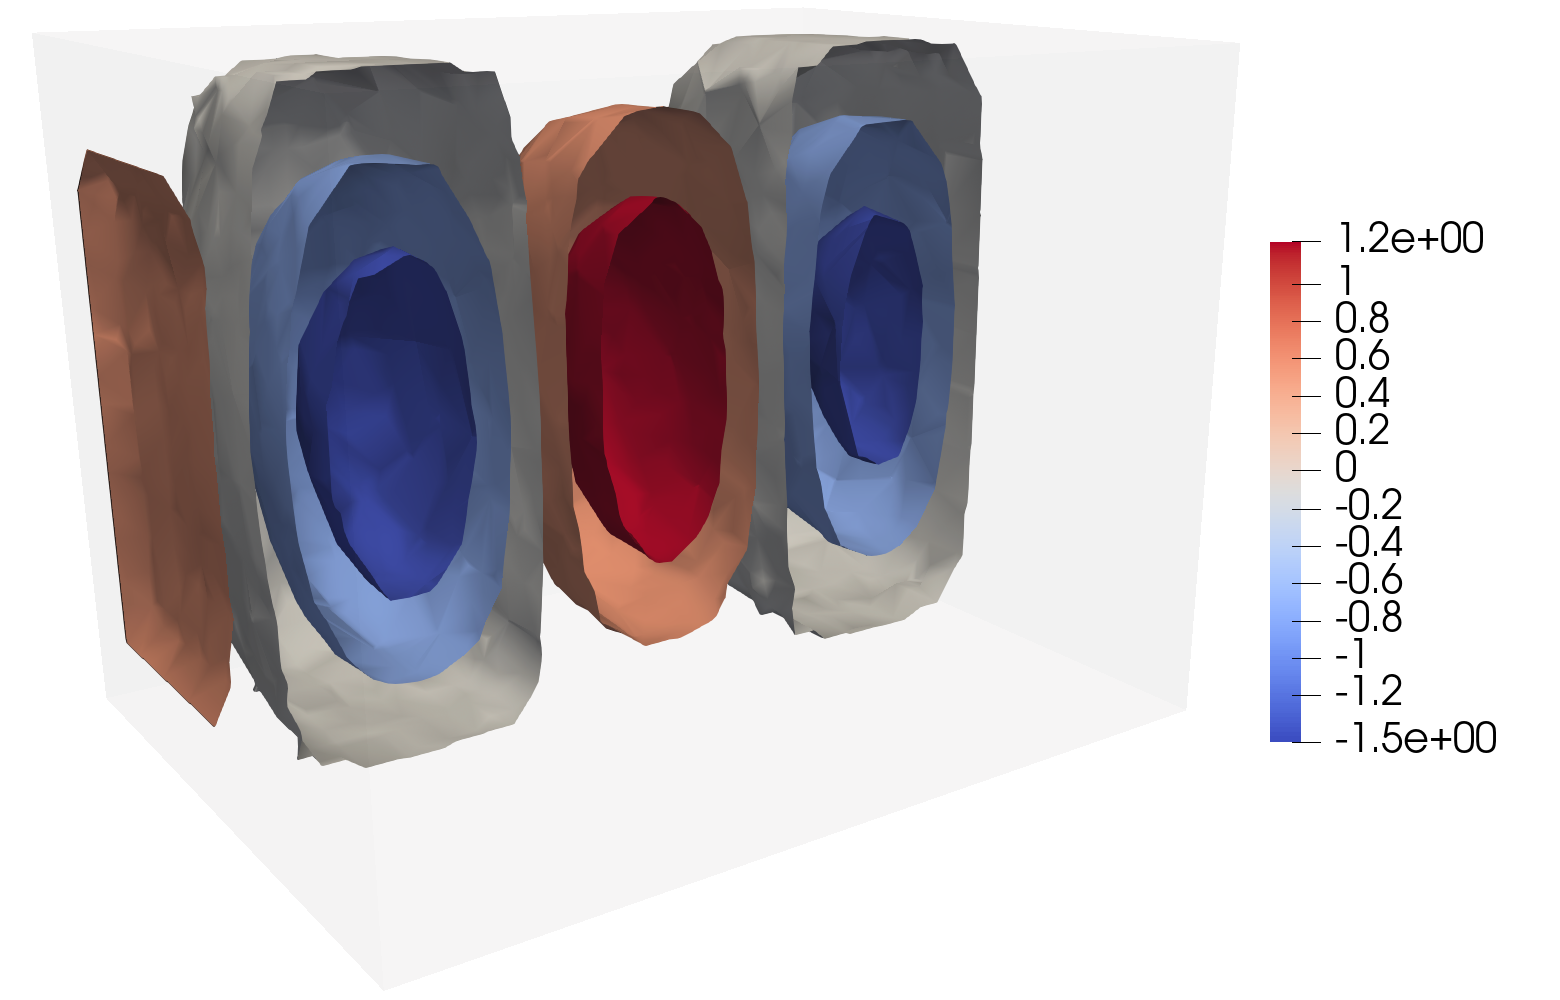
\includegraphics[scale=0.15]{figures/helmholtz/helmholtz_reel_vide3.png}
        \caption{Partie réelle}
    \end{subfigure}%
    \begin{subfigure}{.5\textwidth}
        \centering
        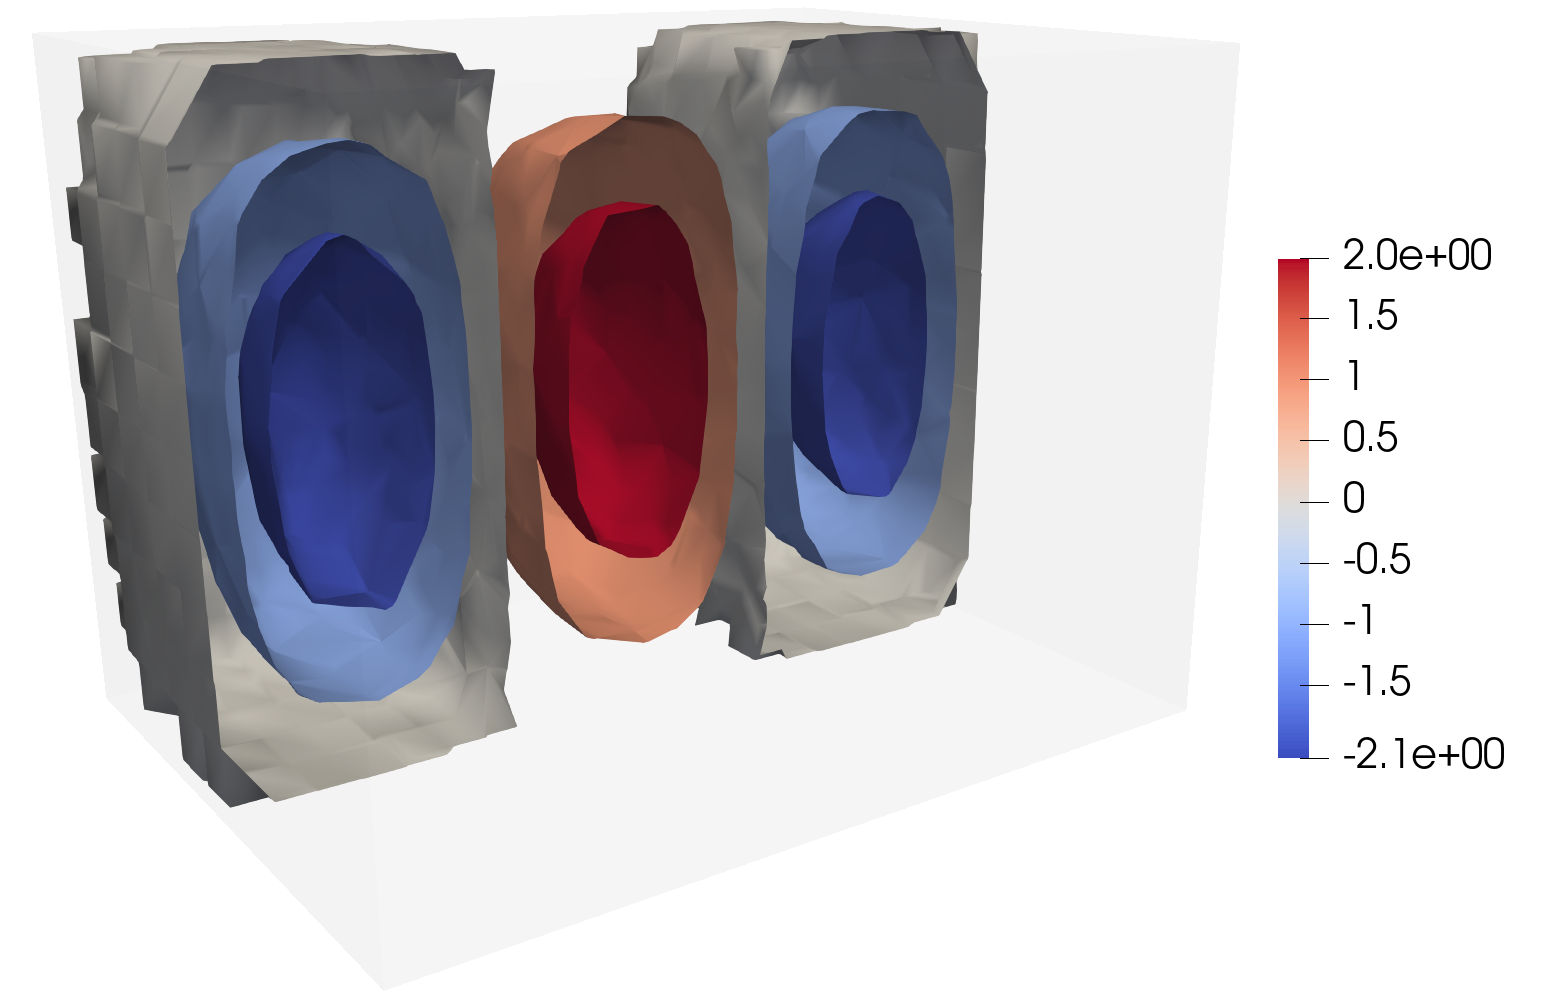
\includegraphics[scale=0.15]{figures/helmholtz/helmholtz_imag_vide3.png}
        \caption{Partie imaginaire}
    \end{subfigure}
    \caption{Des clips des tracés de contours de la magnitude du champ
    électromagnétique dans l'enceinte du four vide. Le clip est au milieu du
    four dans le plan $x\text{-}y$.}
\end{figure}

% ============================================================================

\subsection{Four avec l'aliment dedans}

\begin{figure}[H]
    \centering
    \begin{subfigure}{.5\textwidth}
        \centering
        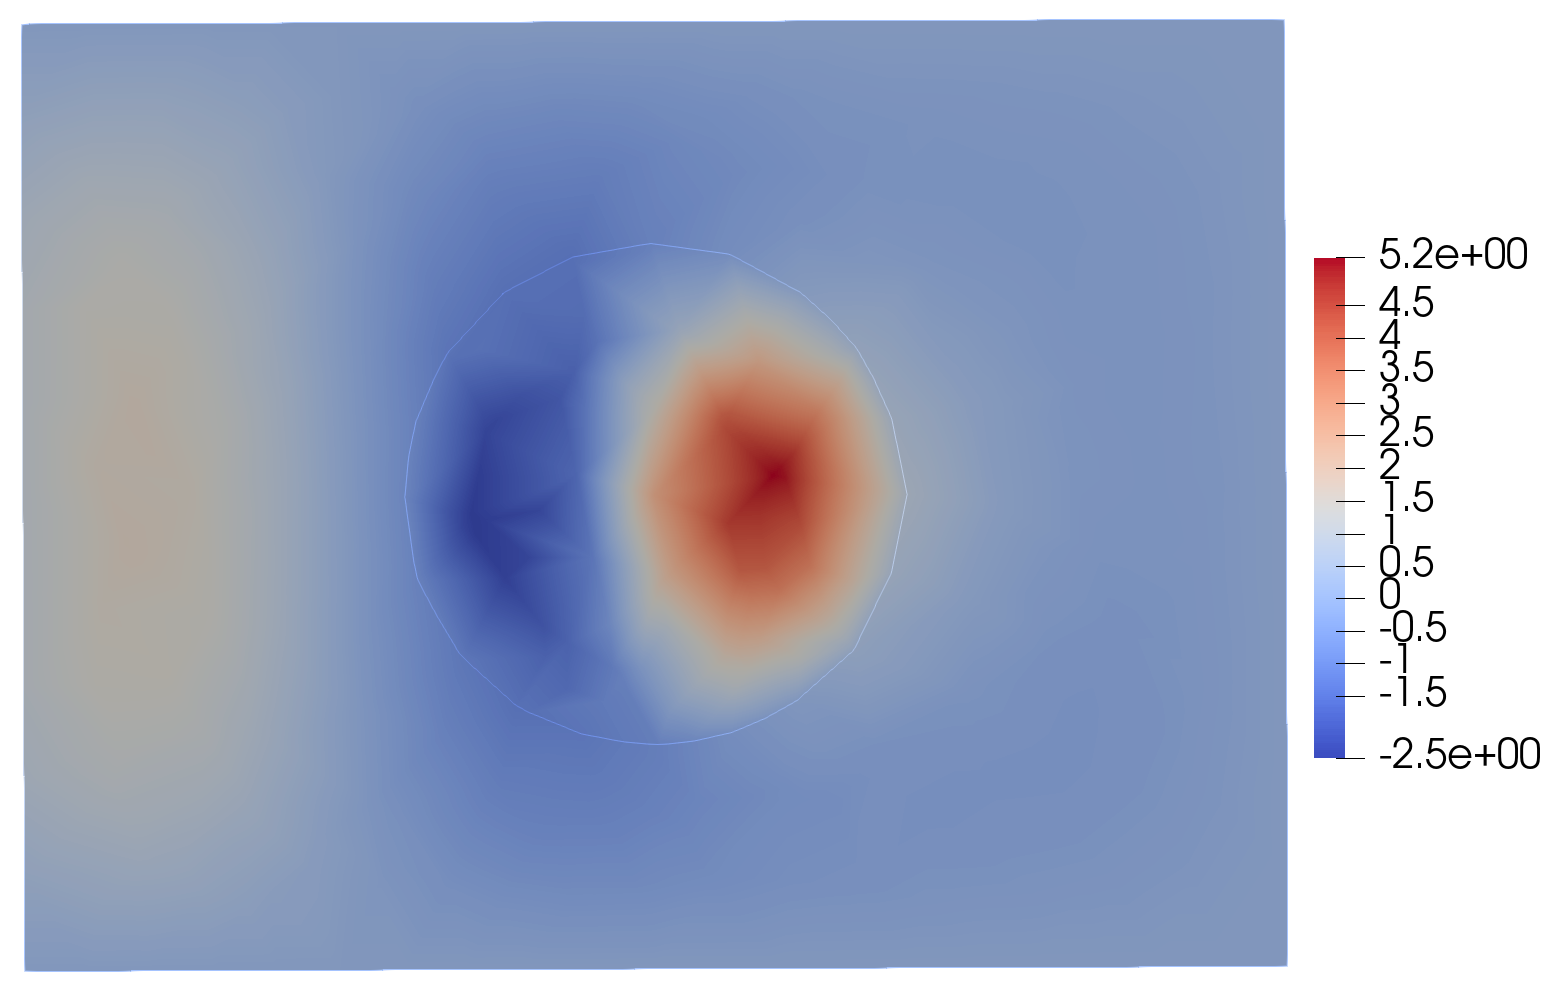
\includegraphics[scale=0.15]{figures/helmholtz/helmholtz_reel1.png}
        \caption{Partie réelle}
    \end{subfigure}%
    \begin{subfigure}{.5\textwidth}
        \centering
        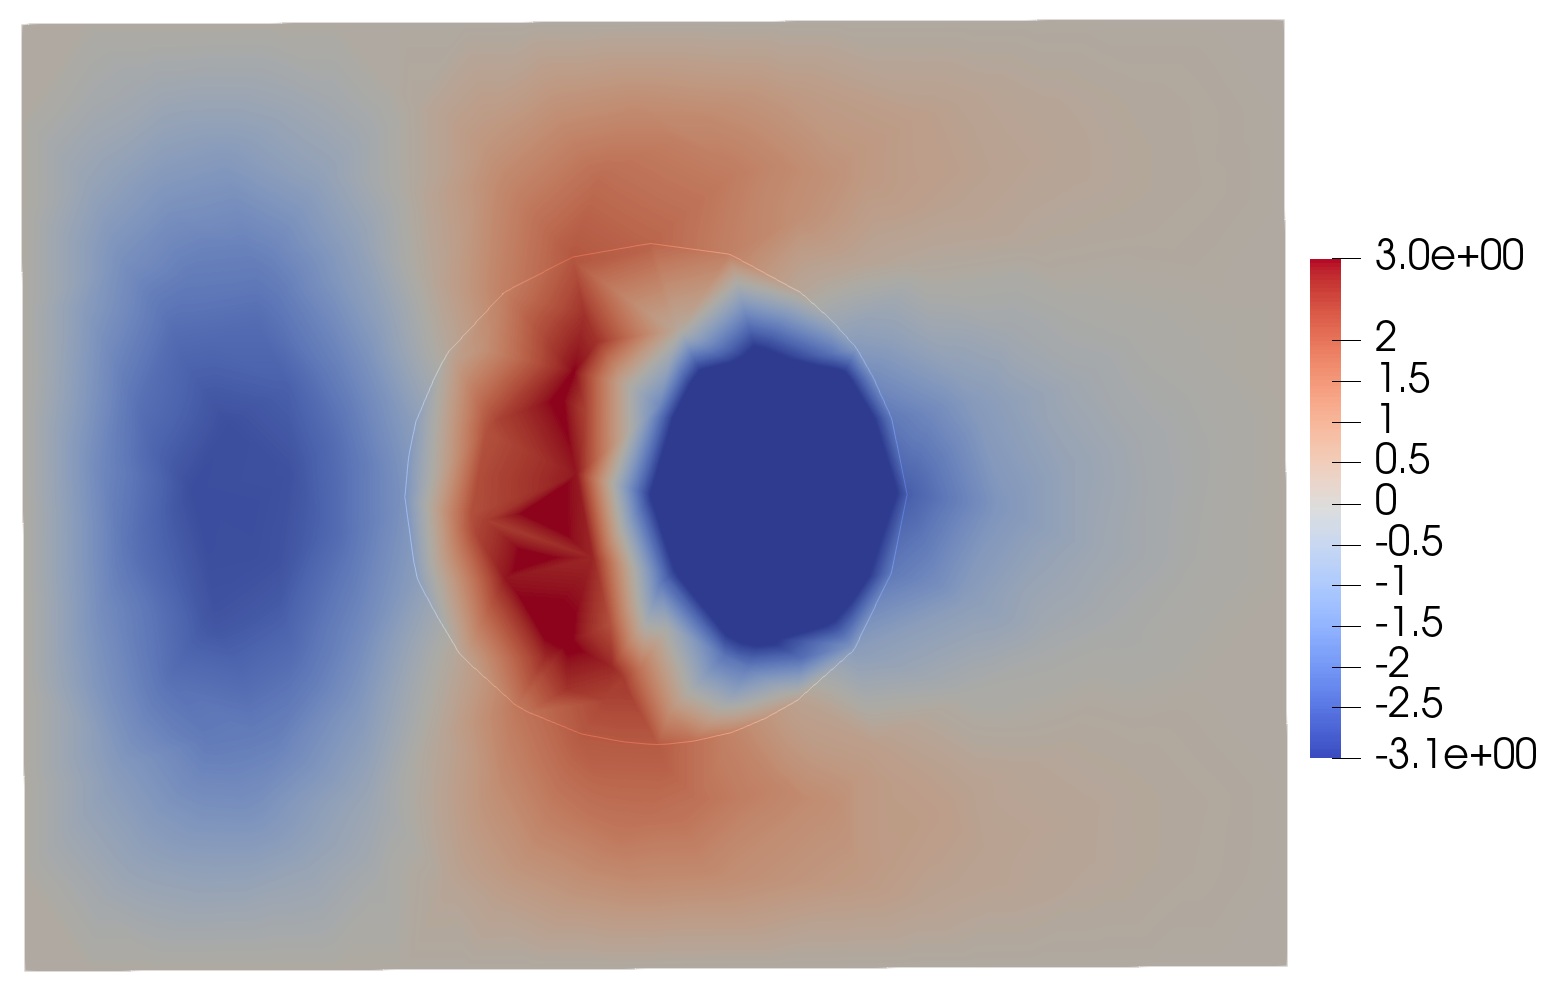
\includegraphics[scale=0.15]{figures/helmholtz/helmholtz_imag1.png}
        \caption{Partie imaginaire}
    \end{subfigure}
    \caption{Une tranche de la magnitude du champ électromagnétique dans l'enceinte
    du four avec l'aliment dedans. La tranche est orientée selon l'axe $x$.}
\end{figure}

\begin{figure}[H]
    \centering
    \begin{subfigure}{.5\textwidth}
        \centering
        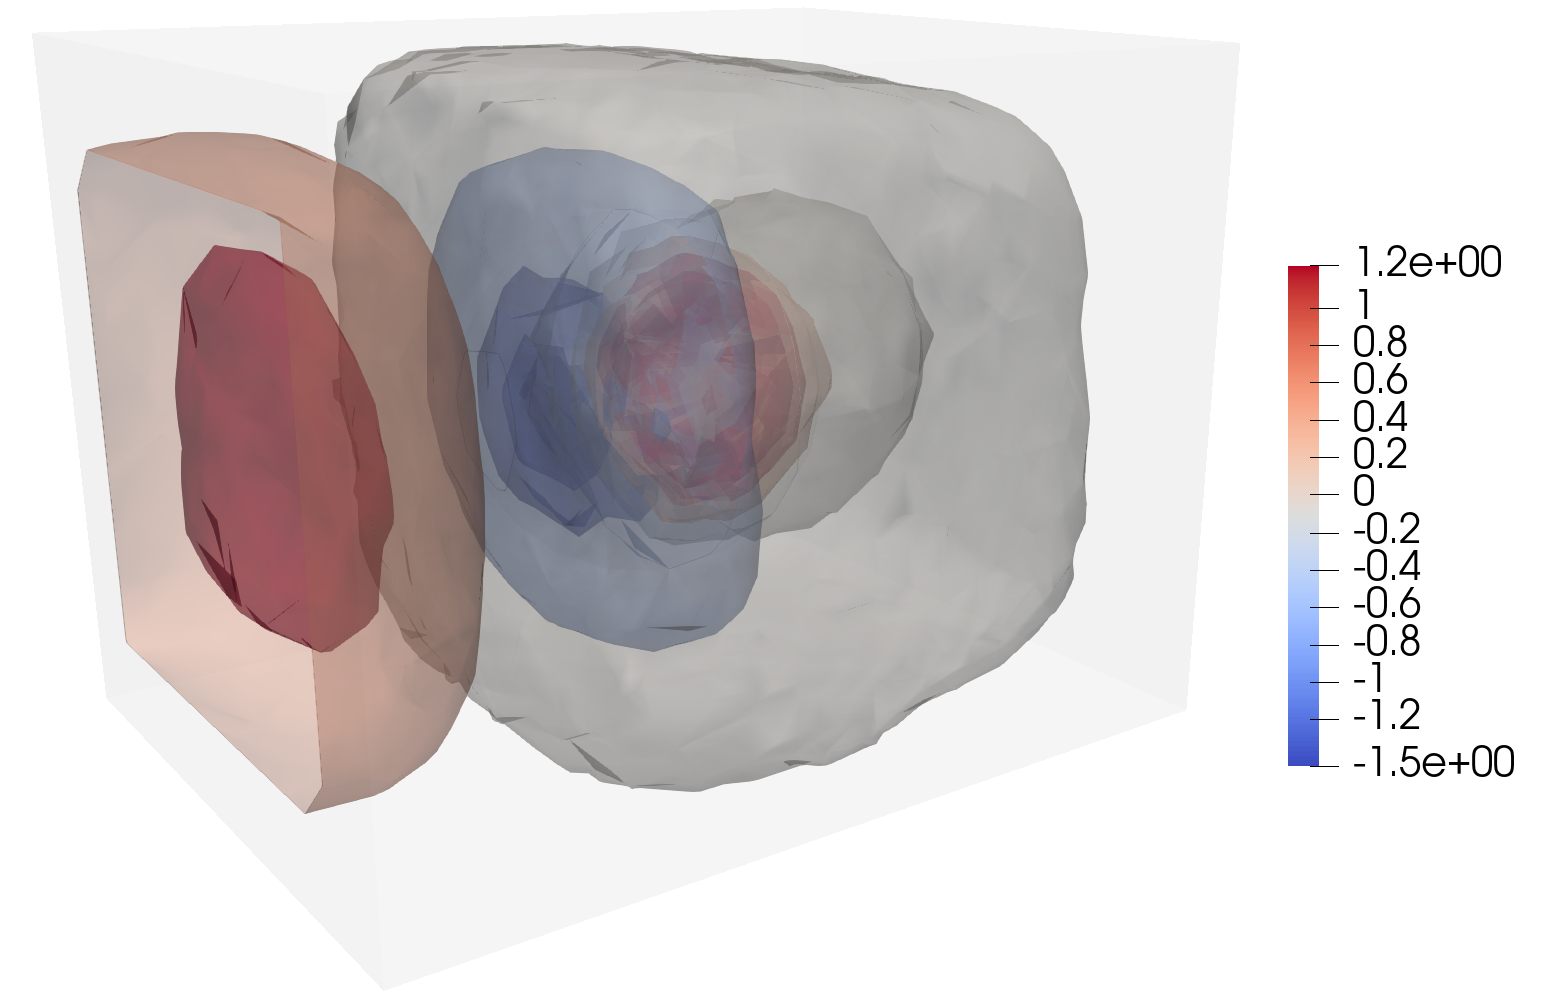
\includegraphics[scale=0.15]{figures/helmholtz/helmholtz_reel2.png}
        \caption{Partie réelle}
    \end{subfigure}%
    \begin{subfigure}{.5\textwidth}
        \centering
        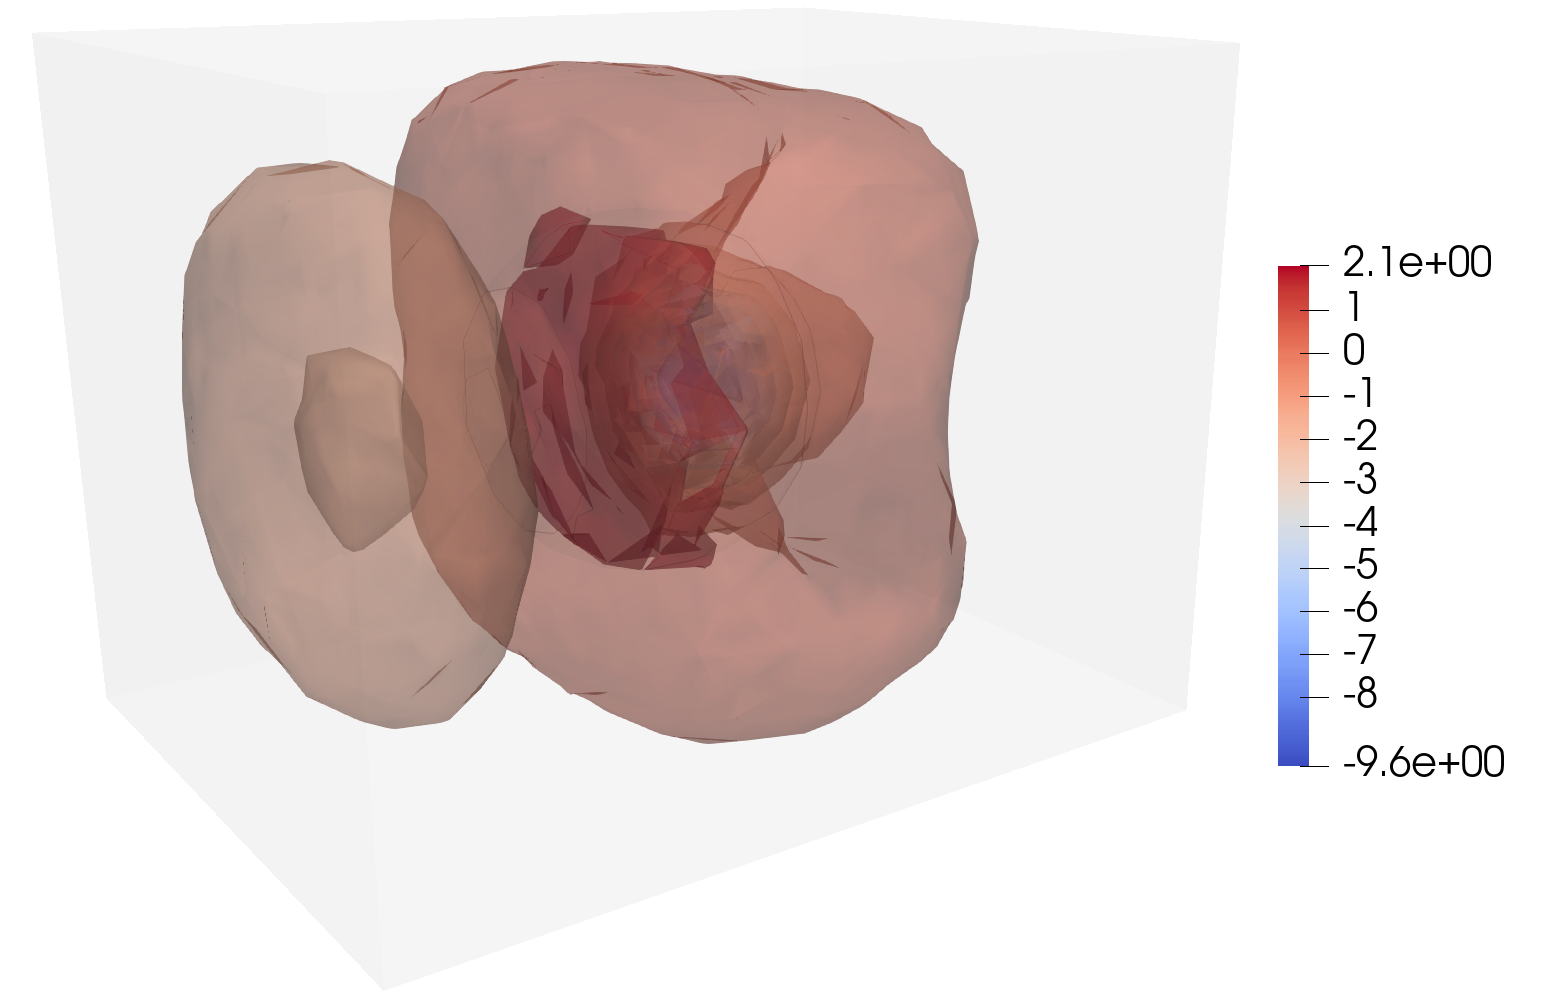
\includegraphics[scale=0.15]{figures/helmholtz/helmholtz_imag2.png}
        \caption{Partie imaginaire}
    \end{subfigure}
    \caption{Des tracés de contours de la magnitude du champ électromagnétique
    dans l'enceinte du four avec l'aliment dedans.}
\end{figure}

\begin{figure}[H]
    \centering
    \begin{subfigure}{.5\textwidth}
        \centering
        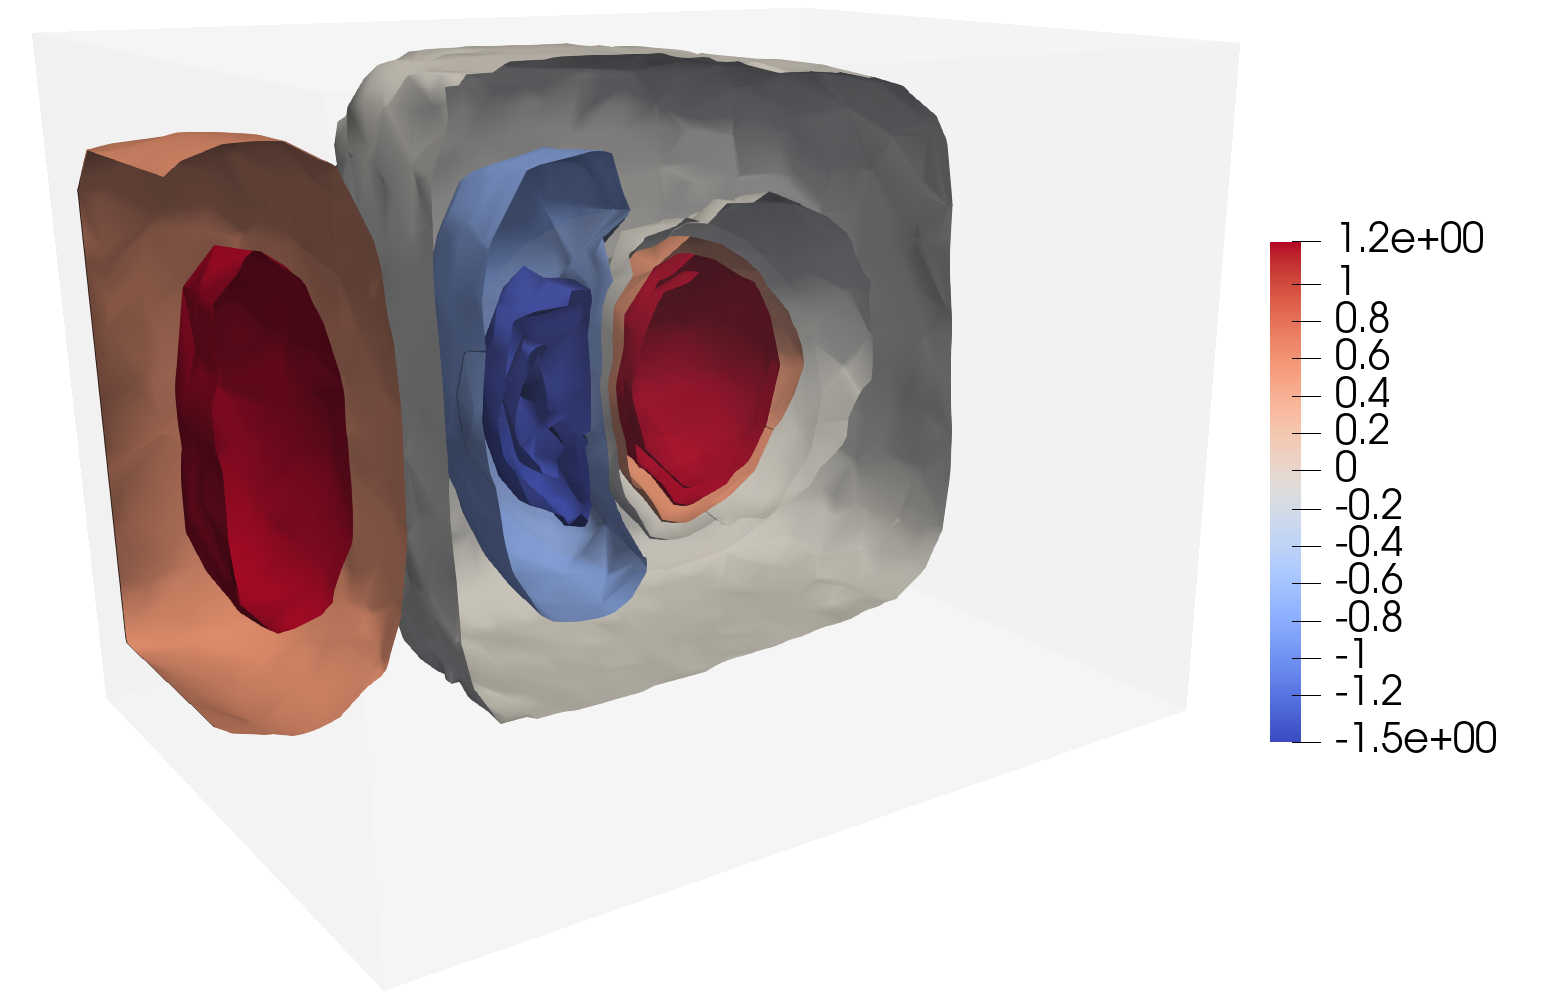
\includegraphics[scale=0.15]{figures/helmholtz/helmholtz_reel3.png}
        \caption{Partie réelle}
    \end{subfigure}%
    \begin{subfigure}{.5\textwidth}
        \centering
        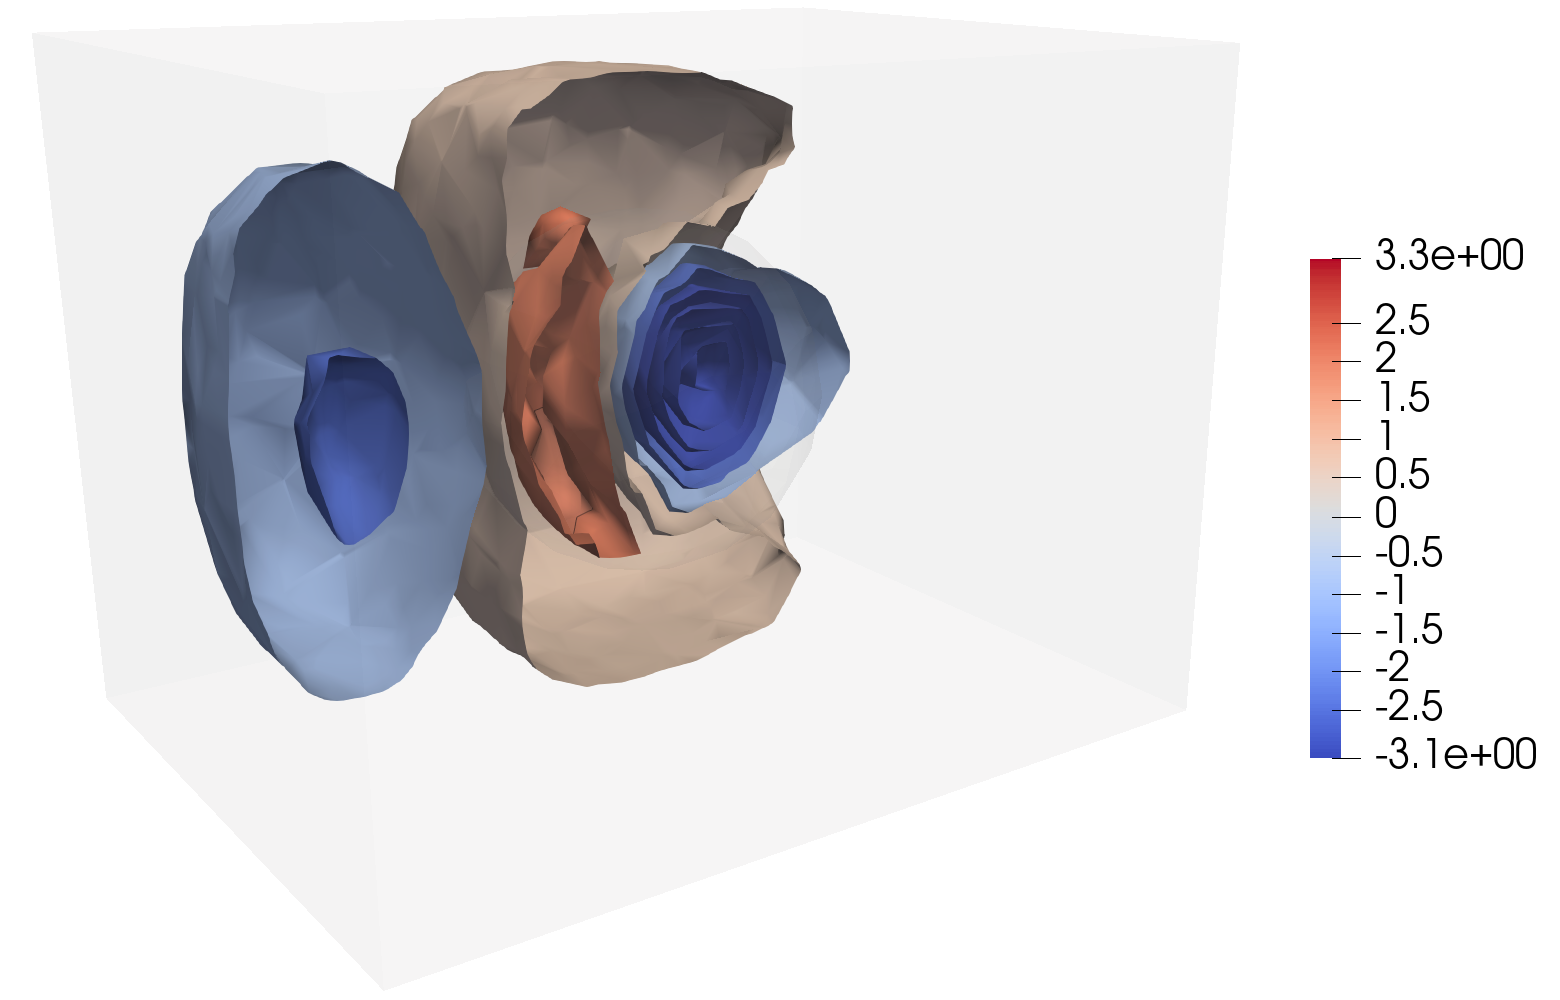
\includegraphics[scale=0.15]{figures/helmholtz/helmholtz_imag3.png}
        \caption{Partie imaginaire}
    \end{subfigure}
    \caption{Des clips des tracés de contours de la magnitude du champ
    électromagnétique dans l'enceinte du four avec l'aliment dedans.
    Le clip est au milieu du four dans le plan $x\text{-}y$.}
\end{figure}
